
\section{Introduction}
\label{sec:introduction}

In this chapter, we make progress towards answering ``What is the most optimal mixing rate in the presence of diffusion for an enstrophy or energy constrained flow?'' This question was also asked in the context of the shell model. We would like to determine if the predictions of the shell model hold in the partial differential equation setting. 

We approach the posed question by considering the general setup, introduced in the introduction chapter, of the evolution of passive scalar in a periodic box. We consider the local-in-time optimization problem introduced by Z. Lin {\it et al.} \cite{JFM2011} in context of pure advection. We now study this optimization problem with the inclusion of diffusion. Local-in-time optimization seeks to find the optimal flow that achieves the best instantaneous mixing rate. We will see that the best choice leads to a $\vec{u}$ that depends on $\theta$. This feedback causes the dynamics of $\theta$ governed by \eqref{eq:PDE_advection} to be nonlinear.

We will demonstrate that homogenization via diffusion and filamentation via advection can sometimes be in conflict and collectively produce a negative impact on mixing. We show numerical evidence that filamentation length scale appears to be limited by the Batchelor scale as seen in the shell model. Even when actively trying to choose the most optimal flow to enhance filamentation. Thus, this may suggest that the Batchelor scale does not only limit turbulent flows but also all incompressible flows under the flow constraints considered here. Although these quantities have been known in the context of turbulence theory, the impact of these limitations on mixing rates has not been fully studied to our knowledge.


The chapter is organized as follows. We introduce the necessary theory regarding local-in-time optimization, a shell model, and $L^{\infty}$ flow constraints in section \ref{sec:theory}. Section \ref{sec:numerical_experiment} details the methodology and results of numerically implementing local-in-time flow optimization. Lastly, we finish with a discussion and conclusion in sections \ref{sec:discussion} and \ref{sec:conclusion} respectively.



%%%
%%%
%%% THEORY
%%%
%%%
\section{Theory}
\label{sec:theory}
\subsection{Local-in-time flow optimization}

We will consider the evolution of a tracer quantity $\theta$ governed by equation \ref{eq:PDE_advection} under an the incompressible flow $\vec{u}$.  Recall the flow is constrained by enstrophy $\ltwo{\nabla\u} = \Gamma L^{d/2}$ or energy $\ltwo{\u} = UL^{d/2}$ where $\Gamma$ is the root mean square rate-of-strain and $U$ is the root mean square speed. 

For the enstrophy-bounded flow problem, we choose the same length scale $L$, the velocity scale $L\Gamma $, and  the time scale $1/\Gamma$. For the energy-bounded flow problem, we non-dimensionalize the system by choosing $L$ as the length scale, $U$ as the velocity scale, and $L/U$ as the time scale.  Both scalings produce the following form of the advection-diffusion equation,
\begin{equation}
\label{eq:nd_ade}
	\ppt{\theta}+\mathbf{u}\cdot \nabla \theta=\frac{1}{Pe} \lap\theta,
\end{equation}
where $Pe=  \frac{\Gamma L^2}{\kappa}$ for the enstrophy-constrained case and $Pe= \frac{UL}{\kappa}$ for the energy-constrained case.   The non-dimensional flow constraints become $\ltwo{\nabla\u} = 1$ or $\ltwo{\u} = 1$.


We consider the local-in-time optimization strategy first introduced by Lin {\it et al.} \cite{JFM2011} in the case without diffusion. We find that this strategy generalizes to the case with diffusion. The local-in-time optimal velocity fields maximize the instantaneous mixing rate by minimizing $\ddt{}\hmone{\theta}^2$. We highlight that local-in-time optimization is not the same as global-in-time or finite-time optimization where the objective is to minimize $\|\theta(\,\cdot\, , T)\|_{H^{-1}}$ at the final time $T$. These objectives generally produce different results.  In the context of the shell model, however, these strategies yielded similar decay rates. The differences between these two objectives under the evolution of  \eqref{eq:nd_ade}  will be the focus of the next chapter and future study. 

The optimal velocity fields are given instantaneously for the enstrophy case by (in non-dimensional form)
%
\begin{equation}
\label{eq:u_lit_enstrophy}
\mathbf{u}= \frac{-\invlap\mathbb{P}(\theta \nabla \invlap\theta)}{\langle |\nabla^{-1}\mathbb{P}(\theta \nabla \invlap\theta)|^2\rangle^{1/2}}
\end{equation}
%
and for the energy case by 
% 
\begin{equation}
\label{eq:u_lit_energy}
\mathbf{u}= \frac{\mathbb{P}(\theta \nabla \invlap\theta)}{\langle |\mathbb{P}(\theta \nabla \invlap\theta)|^2\rangle^{1/2}}
\end{equation} 
%
where $\mathbb{P}$ is the Leray divergence-free projector given by $\mathbb{P}(\vec{v}) = \vec{v} - \nabla \Delta^{-1}(\nabla \cdot \vec{v})$ and $\langle \cdot \rangle$ is the spatial average. These flows will be studied numerically later and is the main focus of this chapter.


We introduce the following measures as useful observables of mixing over time. we use the $H^{-1}$ norm to define the (exponential) rate of mixing as
\begin{equation}
\label{eq:rate}
r(t) = -  \frac{\ddt{}\hmone{\theta}}{\hmone{\theta}}.
\end{equation}
We define the following ratio as a measure of the characteristic filamentation length scale:
\begin{equation}
\lambda(t)\equiv  2\pi \frac{\|\nabla^{-1}\theta(\,\cdot\,,t)\|_{L^{2}}}{\|\theta(\,\cdot\,,t)\|_{L^{2}}}.
\end{equation}
Note that if the tracer concentration field is composed of only one Fourier mode with wave number $\vec{k}$ (i.e. $\theta(\vec{x},t) = Re[ A e^{-i\vec{k}\cdot \vec{x}}]$ where $A$ is a complex constant), then $\lambda(t)$ returns the wavelength of the wave number $\vec{k}$. In general, $\lambda$ is the weighted root mean square wavelength with weights given by $|\theta_{\vec{k}}|^2/\ltwo{\theta}^2$. 


\subsection{Shell model predictions of local-in-time optimization}

The shell model is a model that mimics the spectral dynamics present in the advection-diffusion equation. The model consists of a system of ordinary differential equations with nearest-neighbour coupling between `shells' in wave number space. \cite{Miles2017a} performed local-in-time mixing optimization in this model. The shell-model analysis predicts a limiting length scale given by the Batchelor scale, $\Lambda_{\Gamma} =\sqrt{\frac{\kappa}{\Gamma}}$  and its generalization $\Lambda_{U}= \frac{U}{\kappa} $. The non-dimensional versions are given by $\lambda_{\Gamma}= \frac{1}{\sqrt{Pe}}$ and $\lambda_{U} = \frac{1}{Pe}$. From here forward, we will refer to the Batchelor scale to mean either $\lambda_{\Gamma}$ or its generalization $\lambda_{U}$.  The predicted long-term rates (after reaching the Batchelor scale) are given by $R_{\Gamma} =\kappa/\lambda_{\Gamma}^2 $  and  $R_{U}=\kappa/\lambda_{U}^2$.  The non-dimensional versions are given by $r_{\Gamma} =1$ and $r_{U} = Pe $.

\subsection{Bounds for $L^{\infty}$ constrained flows}
We now consider a subset of $L^{2}$ constrained flows --- those belonging to $L^{\infty}$. In this restricted setting the rate-of-strain and speed are bounded point-wise uniformly in space and time rather than demanding that they merely be $L^2$ integrable as before. Similar analysis of what follows has been attempted in the context of $L^2$ constrained flows, but without success, and appears to be challenging. Thus, we focus on these restricted $L^{\infty}$ constrained subsets of flows where we have been successful at determining bounds on $\lambda$ and measures of mixing. 

\label{sec:linfty_flows}
\subsubsection{Results for $\linf{\nabla \vec{u}} = 1$}

From \eqref{eq:nd_ade}, we find
%
\begin{equation*}
	\frac{1}{(2\pi)^2}\ddt{\lambda^2} = \frac{2}{Pe}
		\left[ 
			\frac{\hone{\theta}^2\hmone{\theta}^2}
					{\ltwo{\theta}^4}  
			- 1
		\right]
		+ 2 \frac{\sint{\nabla^{-1}\theta \cdot \nabla\vec{u} \cdot 
							\nabla^{-1}\theta  }}
					  {\ltwo{\theta}^{2}}
\end{equation*}
and by H\"older's inequality, we deduce
\begin{equation*}
\label{eq:length_ineq_rate-of-strain}
	\frac{1}{(2\pi)^2}\ddt{\lambda^2} \geq \frac{2}{Pe} \left[ 
			\frac{\hone{\theta}^2\hmone{\theta}^2}
					{\ltwo{\theta}^4}  
			- 1
		\right] - \frac{2}{(2\pi)^2}  \lambda^2 .
\end{equation*}
This establishes a lower bound on $\lambda$ at each instant: by apply Gr\"onwall's inequality and the fact that the bracketed term is greater than or equal to zero, it follows that
%
\begin{equation}
\label{eq:exponential_enstrophy}
	\lambda (t) \geq \lambda(0)e^{- t}.
\end{equation}
%


Furthermore,
%
 \begin{eqnarray*}
\frac{d}{dt}\left(\frac{\|\nabla\theta\|_{L^{2}}^2}{\|\theta\|_{L^{2}}^2}\right) &= \frac{\|\theta\|_{L^{2}}^2\frac{d}{dt}\|\nabla\theta\|_{L^{2}}^2-\|\nabla\theta\|_{L^{2}}^2\frac{d}{dt}\|\theta\|_{L^{2}}^2}{\|\theta\|_{L^{2}}^4}\\
&= \frac{-2\sint{\nabla\theta \cdot \nabla\vec{u} \cdot \nabla\theta  } - \frac{2}{Pe} \|\Delta\theta\|_{L^{2}}^2}{\|\theta\|_{L^{2}}^2}+\frac{2}{Pe}\frac{\|\nabla\theta\|_{L^{2}}^4}{\|\theta\|_{L^{2}}^4} \\
&=-\frac{2}{Pe}\left(\frac{\|\Delta\theta\|_{L^{2}}^2}{\|\theta\|_{L^{2}}^2} - \frac{\|\nabla\theta\|_{L^{2}}^4}{\|\theta\|_{L^{2}}^4} \right) - 2\frac{\sint{\nabla\theta \cdot \nabla\vec{u} \cdot \nabla\theta  }}{\|\theta\|_{L^{2}}^2} 
\\
&\leq 2 \frac{\hone{\theta}^2}{\ltwo{\theta}^2}
\end{eqnarray*}
%t
and using $\ddt{}\ltwo{\theta}^2 = -\frac{2}{Pe} \hone{\theta}^2$, it follows that
\begin{equation}
\ltwo{\theta}\geq  \ltwo{\theta_{0}}\exp\left[-\frac{1}{2Pe}\frac{\hone{\theta_{0}}^2}{\ltwo{\theta_{0}}^2}\left(e^{2 t} -1\right)\right].
\end{equation}
Using this with \eqref{eq:exponential_enstrophy}, we deduce the double exponential lower bound
\begin{equation}
\hmone{\theta} \geq  \hmone{\theta_{0}} \exp\left[- t -\frac{1}{2 Pe}\frac{\hone{\theta_{0}}^2}{\ltwo{\theta_{0}}^2}\left(e^{2 t} -1\right)\right].
\end{equation}
Therefore, perfect mixing in finite time is impossible for bounded rate-of-strain flows.

\subsubsection{Results for $\linf{\u}= 1$}
Here we follow and refine an analysis of Poon \cite{Chi-Cheu1996} to show that the presence of diffusion also rules out perfect mixing in finite time for bounded velocity flows as well.  First note that
%
\begin{eqnarray*}
	 \hone{\theta}^2 &=& - 2\sint{\theta \lap \theta} \\
	 							&=& Pe \sint{\theta\left(\ppt{\theta}
	 									-\frac{1}{Pe}\lap \theta\right)} 
	 									-Pe \sint{\theta\left(\ppt{\theta}
	 									+\frac{1}{Pe}\lap \theta\right)},
\end{eqnarray*}
%
\begin{eqnarray*}
	\ddt{}\ltwo{\theta}^2 &=& 2\sint{\theta\ppt{\theta}} \\
										 &=&\sint{\theta\left(\ppt{\theta}
	 									-\frac{1}{Pe}\lap \theta\right)} 
										 + \sint{\theta\left(\ppt{\theta}
	 									+\frac{1}{Pe}\lap \theta\right)} ,
\end{eqnarray*}
%
and
%
\begin{eqnarray*}
	\ddt{}\hone{\theta}^2 &=& -2\sint{\ppt{\theta}\lap \theta} \\
	 									&=& Pe \sint{\left(\ppt{\theta}
	 									-\frac{1}{Pe}\lap \theta\right)^2} 
	 									-Pe \sint{\left(\ppt{\theta}
	 									+\frac{1}{Pe}\lap \theta\right)^2} .
\end{eqnarray*}
%
Then simplify and compute:
%
\begin{eqnarray*}
	\ddt{} \pbrac{ \frac{\hone{\theta}^2}{\ltwo{\theta}^2} } 
			&=& \frac{1}{\ltwo{\theta}^4}
			\sbrac{
				\ltwo{\theta}^2\ddt{}\hone{\theta}^2
				-\ddt{}\ltwo{\theta}^2\hone{\theta}^2			
			}\\
			&=& \frac{1}{\ltwo{\theta}^2}
			 \Bigg[ Pe \sint{\left(\ppt{\theta} -\frac{1}{Pe}\lap \theta\right)^2}  \\
 				& & \qquad\qquad\qquad \qquad \qquad 
				-Pe\sint{\left(\ppt{\theta}+\frac{1}{Pe}\lap \theta\right)^2} 
			\Bigg]\\
		        &-&\frac{1}{\ltwo{\theta}^4}
			\Bigg[ 
				Pe \pbrac{\sint{\theta\left(\ppt{\theta}-\frac{1}{Pe}\lap \theta\right)} }^2\\
 				& & \qquad\qquad\qquad \qquad
				-Pe\pbrac{
					 \sint{\theta\left(\ppt{\theta}
	 									+\frac{1}{Pe}\lap \theta\right)} 
 				}^2					
			\Bigg].
\end{eqnarray*}
%
Using H\"older's inequality and \eqref{eq:nd_ade}, this simplifies to the observation originally noted by Poon \cite{Chi-Cheu1996}:
%
\begin{eqnarray}
	\ddt{} \pbrac{ \frac{\hone{\theta}^2}{\ltwo{\theta}^2} } 
			&\leq & \frac{Pe}{\ltwo{\theta}^2}
			\sbrac{
					 \sint{(\vec{u}\cdot \nabla \theta)^2} 
			}.
\end{eqnarray}
Now applying H\"older's inequality again we have
\begin{equation}
\label{eq:k2growth_energy}
	\ddt{} 
		\pbrac{ 
			\frac{\hone{\theta}^2}{\ltwo{\theta}^2} 
		} 
		\leq  
		Pe
		\frac{\hone{\theta}^2}{\ltwo{\theta}^2} 
\end{equation}
%
and thus 
%
\begin{equation*}
		\frac{\hone{\theta}}{\ltwo{\theta}} 
		\leq  
		\frac{\hone{\theta_0}}{\ltwo{\theta_0}}
		\exp{\pbrac{\frac{Pe}{2} t}}.
\end{equation*}
%
The inequality $\hone{\theta}\hmone{\theta}\geq \ltwo{\theta}^2$ then ensures that
%
\begin{equation}
\label{eq:lambda_bound}
\lambda(t) \geq  2\pi\frac{\ltwo{\theta_0}}{\hone{\theta_0}}\exp{\pbrac{-\frac{Pe}{2}t}}.
\end{equation}
%
Using \eqref{eq:k2growth_energy} together with  $\ddt{}\ltwo{\theta}^2 = -\frac{2}{Pe} \hone{\theta}^2$ we observe that
%
\begin{equation*}
\ltwo{\theta}\geq \ltwo{\theta_{0}}\exp\left[-\frac{1}{Pe^2}\frac{\hone{\theta_0}^2}{\ltwo{\theta_0}^2}\left(e^{Pe \, \, t}-1\right)\right]
\end{equation*}
%
and this combined with  \eqref{eq:lambda_bound} implies another (distinct) double exponential
%
\begin{equation}
\hmone{\theta}\geq \frac{\ltwo{\theta_{0}}^2}{\hone{\theta_0}}\exp\left[-\frac{Pe}{2} \,\, t-\frac{1}{Pe^2}\frac{\hone{\theta_0}^2}{\ltwo{\theta_0}^2}\left(e^{Pe \,\, t}-1\right)\right].
\end{equation}


\section{Numerical experiment: local-in-time optimization}
\label{sec:numerical_experiment}
\subsection{Methodology}


We solve \eqref{eq:nd_ade} with either flow \eqref{eq:u_lit_enstrophy} or \eqref{eq:u_lit_energy} by using a Fourier basis to represent the discretized spatial domain with a 4th order Runge-Kutta time-stepping method.  We slightly perturb the concentration field $\theta_{0}(\mathbf{x}) = \sin(2\pi x/L)$ by evolving the field according to (3) with a steady sin flow given by $\mathbf{u}(\mathbf{x})= \sin(2\pi y/L) \hat{x}$ for a time duration of $0.01$. The concentration field, resulting from this short time integration, is then used as an initial condition for the local-in-time optimization scheme. This perturbation is necessary since the denominator is zero in both expressions (4) and (5) for pure Fourier modes such as $\theta_0$ [2]. The number of Fourier modes is chosen large enough to resolve the spatial resolution and give by the following criteria $N = \min\left[ 2^{ceil(log_2(4(M-1) + 6))} , 512 \right]$ where $M = L/(0.25 \lambda_{B})$ and $\lambda_{B}$ is the appropriate Batchelor scale; The choice of $N = 2^{ceil(log_2(4(M-1) + 6))}$ is suggested as a rule-of-thumb by Ref. \cite{Boyd2000}. The cap of $512$ is suitable for the range of Pe values considered --- the Batchelor wavenumber $k_{B} = 2\pi/\lambda_{B}$ is well within the range of Fourier modes present even after considering $2/3$ dealiasing. The time step is chosen by the CFL condition $dt = 0.25\min\left[L/(UN) , L^2/(\kappa N^2)\right]$ for the enstrophy-constrained case and $dt = 0.25\min\left[1/(\Gamma N) , L^2/(\kappa N^2)\right]$ for the energy-constrained case. All simulation code was created in the programming language Python with package modules, pyfftw and numpy. The code is provided in Appendix \ref{app:lit}.


%%%
%%%
%%% RESULTS
%%%
%%%


\subsection{Results}

\begin{figure}
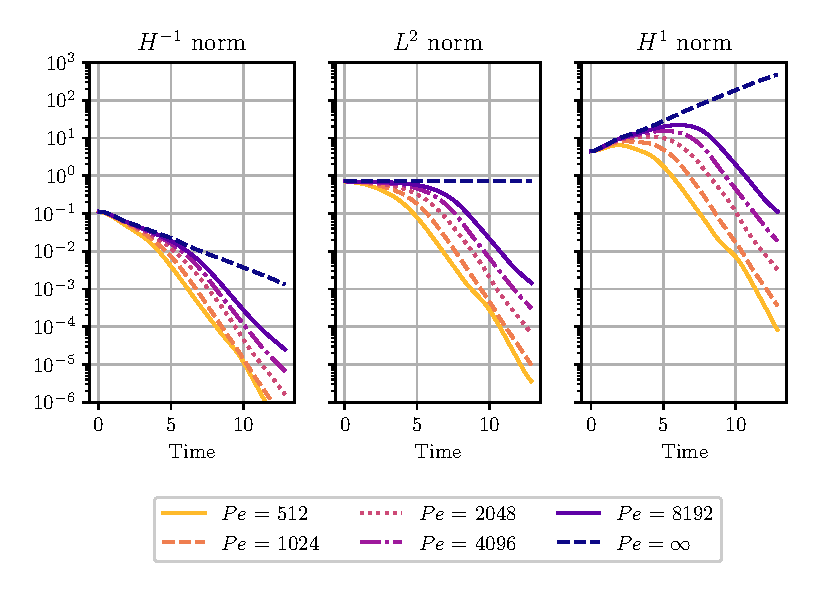
\includegraphics[width=\textwidth]{ch-lit/images/enstrophy_norms}
\caption{$H^{-1}, L^{2},$ and $H^{1}$ norms of the concentration field under the optimal enstrophy-constrained flow.  }
\label{fig:enstrophy_norms}
\end{figure}
%
\begin{figure}
\centering
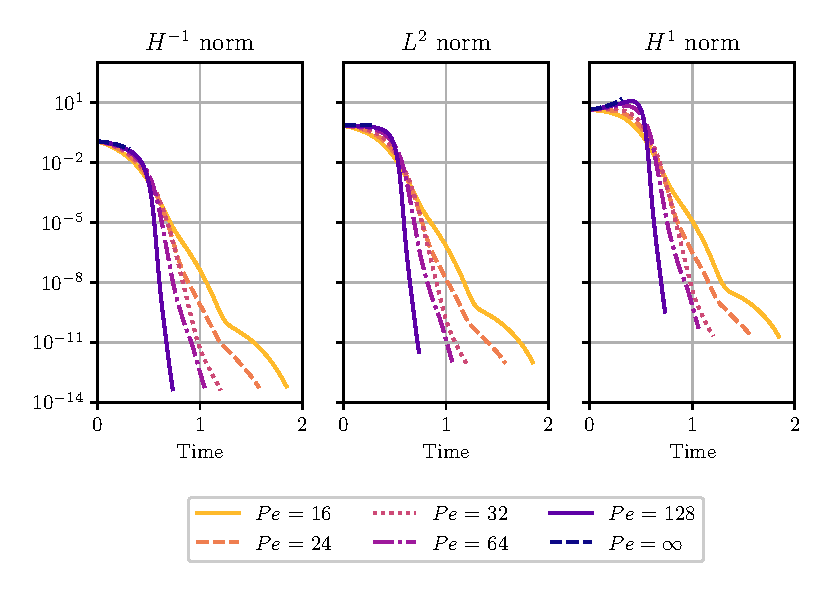
\includegraphics[]{ch-lit/images/energy_norms}
\caption{$H^{-1}, L^{2},$ and $H^{1}$ norms of the concentration field under the optimal energy-constrained flow.}
\label{fig:energy_norms}
\end{figure}


We now investigate the mixing performance under the local-in-time optimal flows. Figure \ref{fig:enstrophy_norms} and \ref{fig:energy_norms} show how the different mixing measures ($H^{-1}$, $L^2$, and $H^{1}$ norms) vary in time for different values of $Pe$ for the enstrophy and energy constrained cases respectively. Notice how the long-term mixing rate appears to be exponential for all three mixing measures. This exponential rate is consistent with shell model predictions, yet weaker than the double-exponential decay rate derived by the $L^{\infty}$ constrained flow analysis.

\begin{figure}
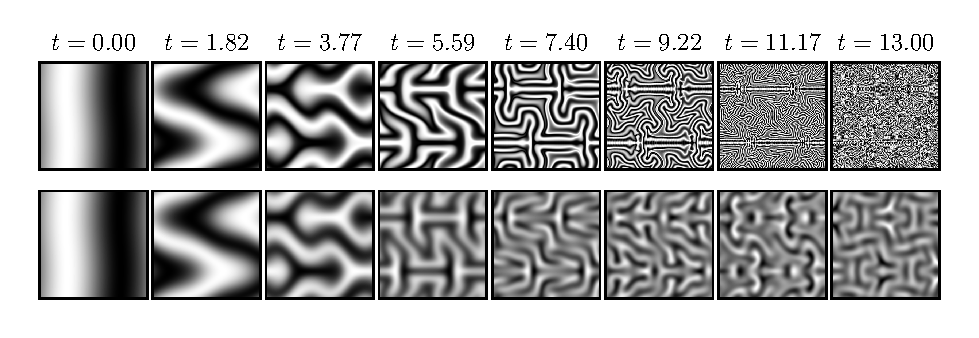
\includegraphics[]{ch-lit/images/enstrophy_film}
\caption{Local-in-time optimization with enstrophy constraint. Top filmstrip is for $Pe =\infty$ and the bottom filmstrip is $Pe=2048$. Note that the grey-scale for the $Pe=\infty$ is constant in time while it is adjusted to show the tracer concentration structure in the finite $Pe$ case. }
\label{fig:enstrophy_film}
\end{figure}
%
\begin{figure}
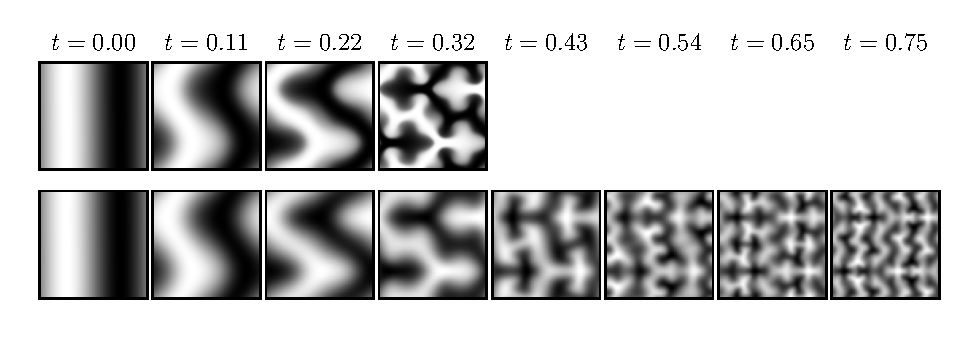
\includegraphics[]{ch-lit/images/energy_film}
\caption{Local-in-time optimization with energy constraint. Top filmstrip is for $Pe = \infty$ and the bottom filmstrip is $Pe=32$. Note that the grey-scale for the $Pe=\infty$ is constant in time while it is adjusted to show the tracer concentration structure in the finite $Pe$ case. The numerical computation is truncated at time $t=0.34$ due to length scales rapidly decreasing past the grid size resolution immediately after $t=0.34$. Fixed energy constrained flows that produce infinitesimally small lengths in finite time have been constructed \cite{JMP2012}. We suspect that the same phenomena may be occurring here.}
\label{fig:energy_film}
\end{figure}
%
\begin{figure}
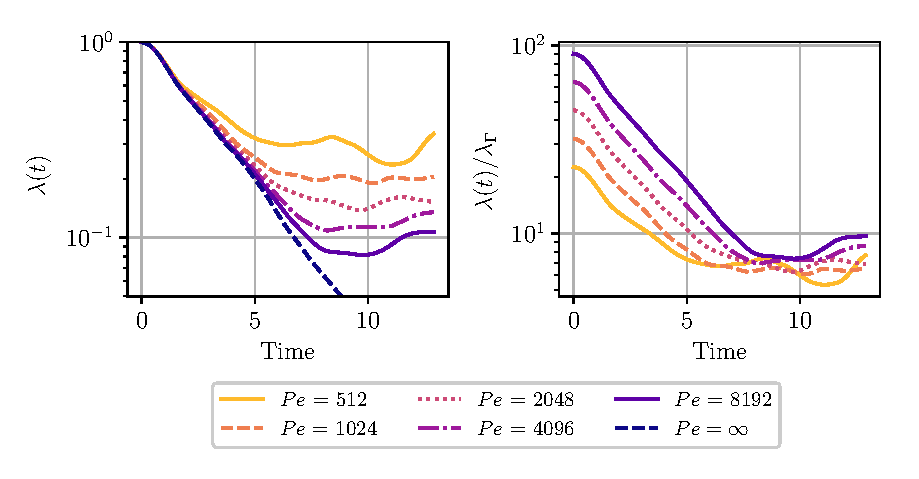
\includegraphics[]{ch-lit/images/enstrophy_length}
\caption{The left subplot shows the filament length $\lambda$ over time subject to the optimal enstrophy-constrained flow. The right subplot is the same data except scaled: $\lambda(t)/\lambda_{\Gamma} = \lambda(t)\sqrt{Pe}$.}
\label{fig:enstrophy_length}
\end{figure}
%
\begin{figure}
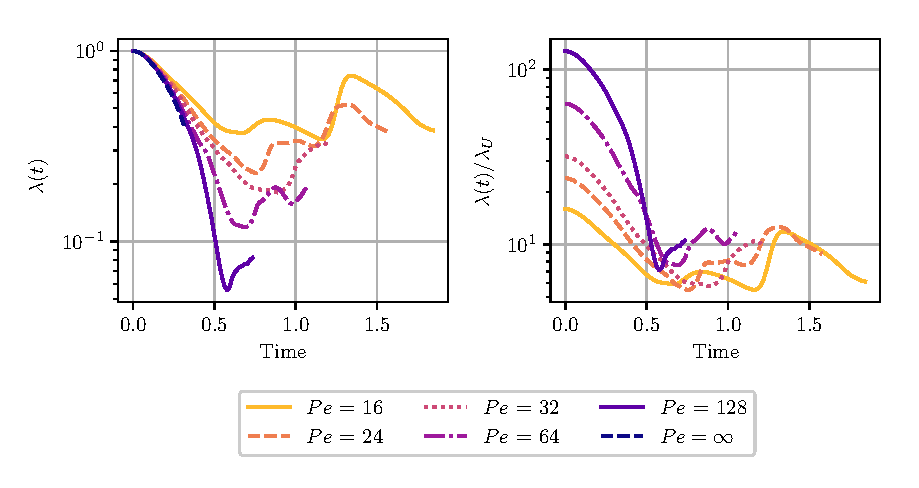
\includegraphics[]{ch-lit/images/energy_length}
\caption{The left subplot shows the filament length $\lambda$ over time subject to the optimal energy-constrained flow. The right subplot is the same data except scaled: $\lambda(t)/\lambda_{U} = \lambda(t) Pe$.}
\label{fig:energy_length}
\end{figure}
%
\begin{figure}
\centering
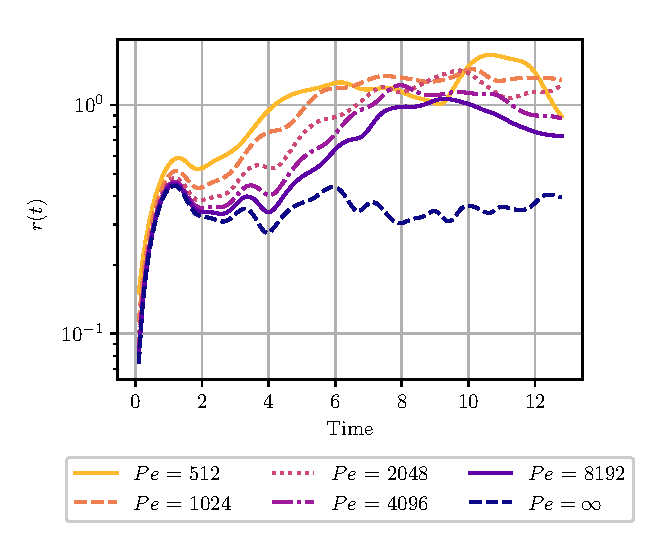
\includegraphics[]{ch-lit/images/enstrophy_rate}
\caption{Mixing rate $r(t)$ over time when subject to the optimal enstrophy-constrained flow.}
\label{fig:enstrophy_rate}
\end{figure}
%
\begin{figure}
\centering
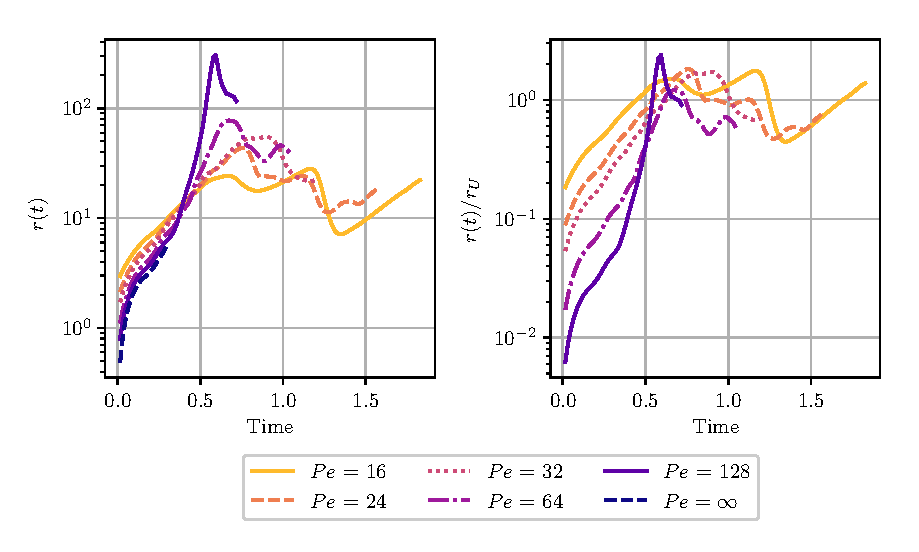
\includegraphics[]{ch-lit/images/energy_rate}
\caption{The left subplot shows the mixing rate $r(t)$ over time when subject to the optimal energy-constrained flow. The right subplot is the same data except scaled: $r(t)/r_{U} = r(t)/Pe$.}
\label{fig:energy_rate}
\end{figure}

 Figure \ref{fig:enstrophy_film} shows the evolution of a scalar field under the optimal flow for the enstrophy constraint. The top film strip corresponds to $Pe =\infty$ while the bottom is $Pe = 256$. The time evolution is initially similar but soon diverges over time. Figure \ref{fig:energy_film} shows the evolution for the energy constraint. The top film strip corresponds to $Pe =\infty$ while the bottom is $Pe = 32$. Notice that, unlike the $Pe = \infty$ cases, the flows with finite $Pe$ are incapable of creating length scales arbitrarily small for either the energy or enstrophy cases.  The left subplot of Figures \ref{fig:enstrophy_length} and \ref{fig:energy_length} shows this phenomena more quantitatively by showing $\lambda$ over time eventually reaching a plateau. The shell-model prediction of this limiting length scale is the Batchelor scale given by $\lambda_{\Gamma} = 1/\sqrt{Pe}$ for the enstrophy case and  $\lambda_{U} = 1/Pe$ for the energy case. The right plots of Figures \ref{fig:enstrophy_length} and \ref{fig:energy_length} shows scaled versions of $\lambda$ given by  $\lambda/\lambda_{\Gamma}$ and $\lambda/\lambda_{U}$ respectively.  Notice how they plateau around an $O(1)$ constant. Thus this result is consistent with the shell-model predictions. 
   
The mixing rates for the enstrophy case are shown in Figure \ref{fig:enstrophy_rate}. The rate during the transient phase is $\Gamma$ which is consistent with rates expected from $Pe=\infty$ mixing studies. For all $Pe$ considered, there is an increase in the rate of mixing after transient behaviour has finished to a long-term rate. Perhaps surprisingly, this long-term mixing rate appears to be {\it independent} of $Pe$ for fixed enstrophy. This suggests that the optimal long-term rate of mixing is only dependent on the rate-of-strain $\Gamma$ and not influenced by the strength of diffusion. 

It should be noted that the onset of the long-term rate is affected by the value of $Pe$. When there is strong diffusion (small $Pe$), the Batchelor scale is reached quickly. From the work of G. Iyer {\it et al.} \cite{GI2014} and C. Seis \cite{CS2013}, we know that $\lambda$ decreases at most exponentially for $Pe = \infty$. If we assume that the local-in-time optimal flows nearly saturate this bound in the transient phase, we model $\lambda$ as  $\lambda (t) = \lambda(0)\exp(- \alpha t) $ during this time. We expect the critical transition time $t_{c}$ that marks the end of this transient period to satisfy $\lambda(t_{c})= \lambda_{\Gamma}$. This time is theorized to be $t_{c}=\frac{1}{\alpha}\ln(\lambda(0)/\lambda_{\Gamma}) = \frac{1}{\alpha}\ln ( \sqrt{Pe} )$ for $Pe>1$ (If $Pe \leq 1$, then there is no transient phase). Hence, a smaller value of $Pe$ will result in an earlier onset of the long-term rate of mixing. Therefore, it is advantageous to have strong diffusion (small $Pe$) so that there is an earlier onset of the long-term mixing rate (although independent of $Pe$) which is an improvement over the mixing rate of the purely non-diffusive situation ($Pe=\infty$).
 
For the energy case, the long-term mixing rate decreases with decreasing $Pe$ (see the left subplot of figure \ref{fig:energy_rate}).  {\it Thus, strong diffusion results in a weak long-term mixing rate}. The right subplot of Figure \ref{fig:energy_rate} is $r/r_{U} =  r/Pe$. We see oscillations of $r/r_{U}$ around a value that is $O(1)$ which indicates that our numerical results are consistent with our predictions from the shell model. Thus, the long-term mixing rate is proportional to $Pe$ in contrast to the long-term mixing rate of enstrophy which carries no dependence on $Pe$.

For the energy case, the onset of the long run-mixing behaviour can be determined by the following model. From the work of E. Lunasin {\it et al.} \cite{JMP2012} on the fixed energy case, $\lambda(t)$ can decrease linearly in time to produce perfect mixing in finite time. We model the transient phase as $\lambda(t)=\lambda(0)(1-\beta t)$. Therefore, we theorize that the critical transition time is $t_{c}=\frac{1}{\beta}(1 -\lambda_{U}/\lambda(0)) = \frac{1}{\beta}(1 - 1/Pe)$ with $Pe> 1$ (If $Pe \leq 1$, there is no transient phase) for the energy case. Thus, it is true that one can still achieve an earlier onset of the long-term mixing behaviour by choosing a smaller $Pe$. However, an earlier onset time is accompanied by a slower long-term mixing rate. As for choosing a large $Pe$, the onset time is bounded above by $\frac{1}{\beta}$ and results in a faster long-term mixing rate. Thus, it is advantageous to have weak diffusion (large $Pe$) for mixing in the fixed energy case. This benefit is well illustrated by $H^{-1}$ norm in figure \ref{fig:energy_norms}. Notice that the mixing rate is initially slow for $Pe = 512$ but then out competes the mixing rate of smaller values of $Pe$.    

%%%
%%%
%%% DISCUSSION 
%%%
%%%

\section{Discussion}
\label{sec:discussion}
%
The local-in-time optimization results suggest that there is a limiting length scale for passive tracer mixing whenever $L^{2}$ flows (either $\ltwo{\mathbf{u}}$ or $\ltwo{\nabla\mathbf{u}}$) are instantaneously optimized to decrease the $H^{-1}$ norm. The bounds derived under both $L^{\infty}$ constrained flow assumptions did not result in proving this observation, but they did definitively rule out the possibility of perfect mixing in finite time for these $L^{\infty}$ flow constraints. 

We suspect that the bounds obtained for $L^{\infty}$ flows are not sharp and could be improved further. The $L^{\infty}$ flow analysis produced a double-exponential lower bound on the $H^{-1}$ norm rather than exponential as possibly expected given the numerical results for local-in-time optimal $L^2$ flows. The double-exponential bounds arise from the use of exponential upper bounds on the quantity $\frac{\hone{\theta}}{\ltwo{\theta}}$ in time for both $L^{\infty}$ flow constraints considered. We surmise that in fact $\frac{\hone{\theta}}{\ltwo{\theta}} < C$ (where $C$ is a constant) for all time $t$ as suggested by the numerical results. If this is true generally for the $L^{\infty}$  flows, then our previous analysis would demonstrate that the $H^{-1}$ norm is bounded below by a single exponential instead of a double exponential.

Note that the pure diffusive case discussed in the introduction can always be employed as a mixing strategy by simply not having a flow field at all ($\vec{u} =\vec{0}$) provided that the flow intensity constraints are generalized to inequalities such as $\|\vec{u}\| \leq UL^{d/2}$ and $\|\nabla \vec{u}\| \leq \Gamma L^{d/2}$. This is a valuable strategy if one is content with mixing at a long-term rate of $\kappa k_{\min}^2$ where $k_{\min} = \min \{ |\vec{k}|  :  |\hat{\theta}_{\vec{k}}(0)| > 0  \}$. This may be advised in fact if $k_{\min} > 2 \pi / \lambda_{B}$. This may well be the most optimal strategy. Invoking a flow may cause the lower wave number modes to become `populated' and therefore may limit the mixing rate. It is important to keep this simple strategy in mind when trying to rigorously prove bounds on the $H^{-1}$ norm. This strategy has an important implication --- there does {\it not} exist a lower bound on the  $H^{-1}$ norm of the form $\hmone{\theta} \geq A e^{-rt}$ where  $r$ is independent of the initial data.

In the next chapter and future work, we will consider the optimal control problem with finite-time optimization to minimize the $H^{-1}$ norm at the end time rather than instantaneously attempting to minimize its decay rate. This might lead to flows that can produce even smaller length scales. In Miles and Doering \cite{Miles2017a}, finite-time optimization was explored in the context of the shell model where it was found that global-in-time and local-in-time optimization appeared to give similar mixing rates. For the shell model, however, the analysis was consistent with computation. In the partial differential equation case, the gap between analysis and computation remains to be closed.


%%%
%%%
%%% CONCLUSION 
%%%
%%%


\section{Conclusion}
\label{sec:conclusion}


Our numerical study of local-in-time optimization suggests that there is a limiting length scale, a generalized Batchelor length scale, which in turn determines a long-term mixing ``Batchelor rate". In dimensional form, this Batchelor rate was found to be proportional to $\Gamma$ for the fixed enstrophy case and $U^{2}/\kappa$ for the fixed energy case. These rates are consistent with those found in the context of the shell model. Although the Batchelor scale has been a theorized lower bound on the length scales present on turbulent flows, it has not been proven rigorously. We hope this numerical study provides insight and promotes investigation into mathematically proving what conditions are necessary on the flow for a length scale limitation. This is especially important since it plays a crucial role in the achievable mixing rates. Furthermore, we provided numerical evidence that (1), for fixed enstrophy optimal flows, strong diffusion can benefit from an early onset of a long-term mixing rate (where the rate itself however is independent of diffusion strength) while (2), for energy fixed optimal flows, strong diffusion weakens the long-term mixing rate. 

 

